\documentclass[a4paper,12pt]{article}
\usepackage[utf8]{inputenc}
\usepackage[ngerman]{babel}
\usepackage[T1]{fontenc}
\usepackage[default]{raleway}
\usepackage{mathtools}
\usepackage[dvipsnames]{xcolor}
\usepackage[marginal, norule, perpage]{footmisc}
\usepackage{tabularx}

\renewcommand{\thefootnote}{\Roman{footnote}}

\usepackage{hyperref}
\hypersetup{
  colorlinks=true,
  linkcolor=MidnightBlue,
  urlcolor=MidnightBlue
}

\title{Angewandte Mathematik\\	\large{Differentialgleichungen und ihre Anwendung}\bigskip\\	\small{Jahrgang 4 - Semester 1 - SA 2}}
\author{Markus Reichl}

\begin{document}

\maketitle

\tableofcontents

\newpage

\section{Einf\"uhrung}
\subsection{Definition}
Eine Differentialgleichung liegt vor, wenn eine gesuchte Gr\"o\ss{}e in mindestens einer Ableitung einer Gleichung vorkommt.
$$y'=3x+1$$
$$y=x^2+x+C$$
Das Ergebnis einer Differentialgleichung ist eine Funktionenschar welche \textbf{Allgemeine L\"osung} genannt wird. 
Diese kommt aufgrund der Vieldeutigkeit (Integrationskonstante C) der Integration zustande und k\"onnen durch eine Nebenbedingung begrenzt werden. Das Resultat nennt man \textbf{Partielle L\"osung}.
$$y'=3x+1 \quad \text{mit} \quad y(0)=1$$
$$y=\frac{3x^2}{2} + x + C$$
$$1=\frac{3*0}{2} + 0 + C \to C = 1$$
$$y=\frac{3x^2}{2}+x+1$$

Wird die Integrationskonstante durch eine Anfangsbedingung festgelegt,
nennt man diese eine Anfangswertaufgabe.
Sind diese an verschiedenen Stellen festgelegt spricht man von einer Randwertaufgabe.
\subsection{Nomenklatur}
DGLs beschreiben die Änderung einer gesuchten Größe.
\\
$y' = dy / dx$\quad' Ableitung nach dem Ort x (Ortsangabe)\\
$y^\circ = dy / dt$\quad$^\circ$ Ableitung nach der Zeit t (Zeitangabe)

\paragraph{Ordnung} Die Ordnung einer DGL gibt die höchste auftretende Ableitung an.\\
\texttt{Bsp.: $y'' \to$}\quad DGL 2. Ordnung
\paragraph{Grad} Der Grad einer DGL gibt die höchste auftretende Potenz an, einschließlich ihrer Ableitungen.\\
\texttt{Bsp.: $y'' * 2^3 \to$}\quad DGL 3. Grades\bigskip\\
Ist der 1. der h\"ochste vorkommende Grad handelt es sich um eine lineare Differentialgleichung.

\section{Richtungsfelder}
F\"asst man y' als Funktion in 2 Variablen auf, kann zu jedem (x, y) Paar ein Funktionswert der Richtung ermittelt werden.
$$y' = f(x, y)$$
$$y' = 1 - 2y$$
$$\downarrow$$
\begin{tabular}{l l l}
 $f(0, 1) = -1$ & $f(1, 1) = -1$ & $f(2, 1) = -1$\\
 $f(0, 0) = 1$ & $f(1, 0) = 1$ & $f(2, 0) = 1$\\
 $f(0, 2) = -3$ & $f(1, 2) = -3$ & $f(2, 2) = -3$
\end{tabular}

$$\downarrow$$

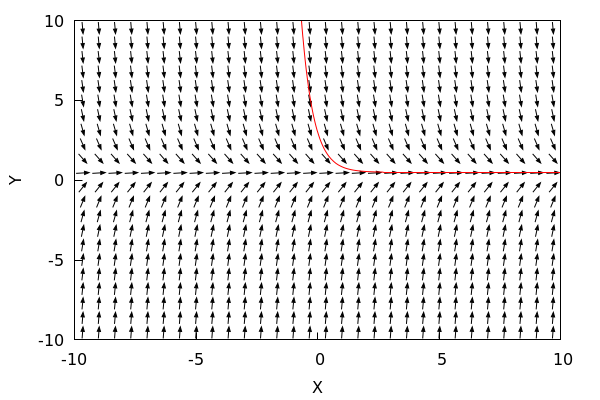
\includegraphics[scale=0.6]{richtungsfeld01.png}

\newpage

\section{Berechnung}
\subsection{Trennung der Variablen}
Separierbare Differentialgleichungen 1. Ordnung lassen sich durch die Methode ``Trennung der Variablen'' l\"osen.
Das Vorgehen ist dabei klar und einfach anzuwenden. Als Beispiel wird die Gleichung $y' + 2*y = 1$ mit der Nebenbedingung $y(0) = 3$ verwendet.
\paragraph{1. Isolieren von y'}
Die Ableitung y' muss zur Aufl\"osung auf eine Seite gebracht werden.
$$y' = 1 - 2*y$$
\paragraph{2. Ersetzung}
y' muss nun durch die Schreibweise $\frac{dy}{dx}$ ersetzt werden.
$$\frac{dy}{dx} = 1 - 2*y$$
\paragraph{3. Trennung}
Nun muss die Gleichung so aufgeteilt werden, dass sich $dy$ auf einer und $dx$ auf der anderen Seite befinden. $dx$ sollte dabei alleine stehen.
$$\frac{dy}{(1-2y)} = dx$$
\paragraph{4. Integration}
Nun m\"ussen beide Seiten einzeln integriert werden:
$$\int\frac{1}{1 - 2y} dy = \int{dx}$$
$$-\frac{1}{2}\log{1 - 2*y} = x + \%c$$
\paragraph{5. Berechnung}
Jetzt kann nach y aufgel\"ost werden und man erh\"alt die \textit{Allgemeine L\"osung}:
$$y_a = \frac{1}{2}*(1-C*e^{-2\,x})$$
\subsection{Einsetzen von Nebenbedingungen}
Wenn eine Nebenbedingung angegeben ist, kann diese in die Allgemeine L\"osung eingesetzt werden. 
Dadurch erh\"alt man einen bestimmten Wert f\"ur die Integrationskonstante $\%c$.
$$y(0) = 3 \to \%c = -5$$
Diese eingesetzt ergibt sich die \textit{Partielle L\"osung}:
$$y_p = \frac{1}{2}*(1+5*e^{-2\,x})$$

\subsection{Anwendung in Maxima}
Die Ableitung y' wird in Maxima unter der Schreibweise $\frac{dy}{dx}$ benötigt, welche man mittels \texttt{'diff(y, x)} erhält:
\begin{verbatim}
 dgl01: 'diff(y, x) + 3*y*cos(x) = 0;        
\end{verbatim}
$${\frac{d}{d\,x}}\,y+3\,\cos x\,y=0$$

Mittels der Funktion \texttt{ode2(equation, var, params)} kann nun nach y aufgelöst werden, wodurch man die allgemeine Lösung erhält:
\begin{verbatim}
 y01a: ode2(dgl01, y, x);
\end{verbatim}
$$y={\it \%c}\,e^ {- 3\,\sin x }$$

Durch Einsetzen der Nebenbedingung in die allgemeine Lösung erhält man einen Wert für die Konstante C:
\begin{verbatim}
 y01nb: solve(1 = subst(0, x, rhs(y01a)));
\end{verbatim}
$$\left[ {\it \%c}=1 \right] $$

Setzt man diesen ein erhält man die spezielle Lösung:
\begin{verbatim}
 y01c: subst(y01nb, y01a);
\end{verbatim}
$$y=e^ {- 3\,\sin x }$$

In Maxima nutzt man für dieses Vorgehen folgende Funktion:
\begin{verbatim}
 ic1(y01a, x=0, y=1);
\end{verbatim}
$$y=e^ {- 3\,\sin x }$$

\section{Anwendung von DGL 1. Ordnung}
\subsection{Wachstumsmodelle}
\subsubsection{Lineares Wachstum}
Beschreibt ein unbeschränktes Wachstum um einen konstanten Faktor.
Die Differentialgleichung lautet:
$$y^\circ      = k$$
In Maxima kann diese Gleichung mittels \texttt{ode2} aufgelöst werden:
$$y(t)    = kt + \%c$$
Die lineare Wachstumsfunktion kann auch explizit dargestellt werden indem man $\%c$ anhand von $y(0)$ bestimmt.
$$y(0) = \%c$$
In die Gleichung eingesetzt erh\"alt man dadurch die explizite Darstellung:
$$y(t)    = y(0) + kt$$

\begin{flushleft}
 \textbf{Grafische Darstellung}
\end{flushleft}
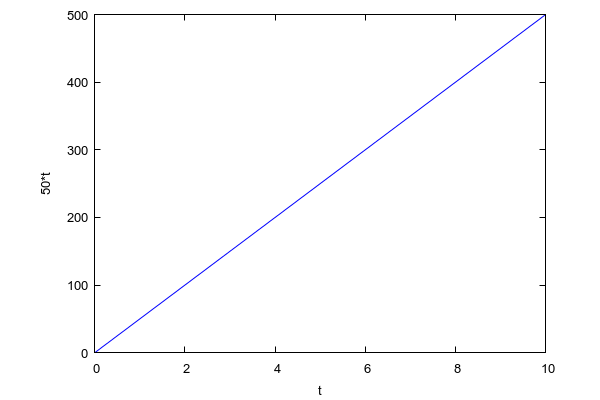
\includegraphics[scale=0.6]{lineares-wachstum.png}

\subsubsection{Exponentielles Wachstum}
Beschreibt ein unbeschränktes Wachstum um eine konstante Wachstumsrate.
Die Differentialgleichung lautet:
$$y^\circ      = k * y$$
In Maxima kann diese Gleichung mittels \texttt{ode2} aufgelöst werden:
$$y={\it \%c}\,e^{k\,t}$$

Die exponentielle Wachstumsfunktion kann auch explizit dargestellt werden indem man $\%c$ bestimmt.
y(0) ergibt genau den Wert der konstante, da die Exponentialfunktion von t abh\"angt und wegf\"allt.
$$y(0) = \%c$$
Nun kann man $\%c$ einsetzen, womit man auf die explizite Darstellung kommt:
$$y(t)    = y(0) * e^{k\,t}$$

\begin{flushleft}
 \textbf{Grafische Darstellung}
\end{flushleft}
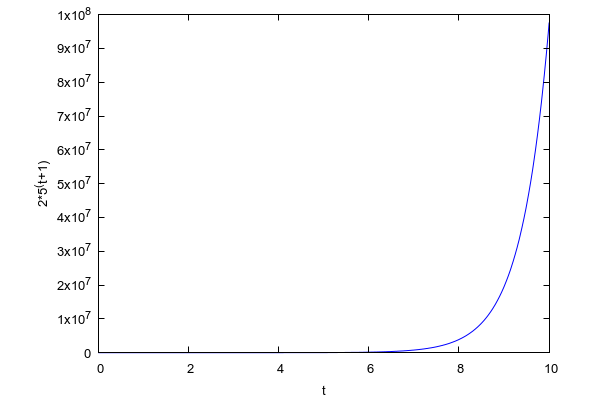
\includegraphics[scale=0.6]{exponentielles-wachstum.png}

\subsubsection{Beschr\"anktes Wachstum}
Beschreibt ein beschränktes Wachstum um eine konstante Wachstumsrate. 
Hierzu gibt es verschiedene Auffassungen, die Differentialgleichung aus dem Unterricht lautet:
$$y^\circ      = k*(1 - \frac{y}{K})$$
\begin{center}
 \small{[k ... Wachstumsrate, K ... Beschr\"ankung]}
\end{center}
In Maxima kann diese Gleichung mittels \texttt{ode2} aufgelöst werden:
$$y={\it \%c}\,e^ {- {\frac{k\,t}{K}} }+K$$

Die exponentielle Wachstumsfunktion kann auch explizit dargestellt werden indem man $\%c$ bestimmt.
Durch die Berechnung von y(0) erkennt man, dass $\%c$ gleich $y(0) - K$ ist.\bigskip
\\
Nun kann man $\%c$ einsetzen, womit man auf die explizite Darstellung kommt:
$$y=e^ {- {\frac{k\,t}{K}} }\,\left({\it y_0}-K\right)+K$$
\begin{flushleft}
 \textbf{Grafische Darstellung}
\end{flushleft}
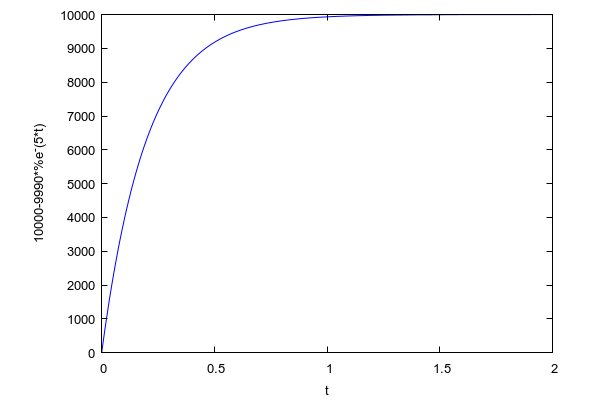
\includegraphics[scale=0.6]{beschraenktes-wachstum.png}

\subsubsection{Logistisches Wachstum}
Beschreibt ein beschränktes Wachstum um eine konstante Wachstumsrate, auf Basis der Population. 
Die Differentialgleichung lautet:
\[y^\circ=k\,\left( K-y\right) y\]
\begin{center}
 \small{[k ... Wachstumsrate, K ... Beschr\"ankung]}
\end{center}
In Maxima kann diese Gleichung mittels \texttt{ode2} aufgelöst werden:
$$\log{\left( \frac{y}{y-K}\right) }=Kk\,\left( t+\mathit{\%{}c}\right)$$
Die logistische Wachstumsfunktion kann auch explizit dargestellt werden indem man $\%c$ \"uber $y(0)$ bestimmt:
$${\it \%c}={{\log \left(-{{{\it y_0}}\over{K-{\it y_0}}}\right)}\over{K\,k}}$$
Nun kann man $\%c$ einsetzen, womit man auf die explizite Darstellung kommt:
$$y=\frac{K\,\mathit{y0}}{{{\%{}e}^{-Kkt}}\,\left( K-\mathit{y0}\right) -\mathit{y0}}$$
Ein sch\"oneres Ergebnis erh\"alt man durch eine h\"andische Variablentrennung:
$$y={{K}\over{e^ {- K\,k\,t }\,\left({{K}\over{{\it y_0}}}-1\right)+1}}$$

\newpage

\begin{flushleft}
 \textbf{Grafische Darstellung}
\end{flushleft}
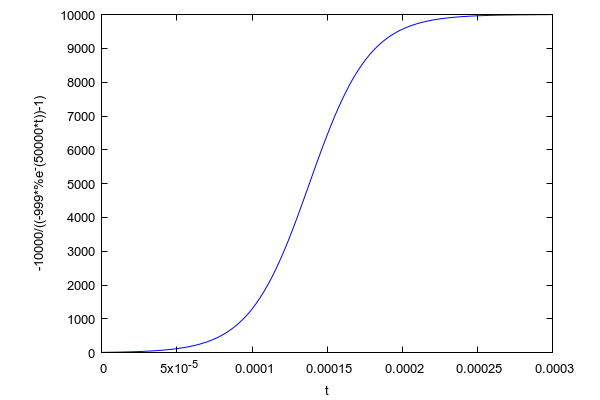
\includegraphics[scale=0.6]{logistisches-wachstum.png}

\subsubsection{Andere Auffassungen}
\paragraph{Beschr\"anktes Wachstum}~\\
Quasi identische Ergebnisse erh\"alt man mit folgender Differentialgleichung:
$$y^\circ = k*(K - y)$$
Bei gleichem Vorgehen kommt man auf eine L\"osung von:
$$y={\it \%c}\,e^ {- {k\,t} }+K$$
Sowie eine explizite Darstellung von:
$$y=e^ {- {k\,t} }\,\left({\it y_0}-K\right)+K$$

\newpage

\subsection{Physik}
Kräfte in der Physik können häufig durch Differentialgleichungen beschrieben werden, hier nur ein paar Beispiele:
\[v=\frac{d}{dt}s \to s = \int v * dt\]
\[a=\frac{d}{dt}v \to v = \int a * dt\]
\[F = m*a = m*\left( \frac{d}{dt}v\right) \]

\newpage

\section[Lineare DGL 1. Ordnung mit konstanten Koeffizienten]{Lineare Differentialgleichungen 1. Ordnung\\ mit konstanten Koeffizienten}
Die Lösung einer linearen DGL 1. Ordnung mit konstantem Koeffizienten p (y' + p * y = s(x)) kann immer aus der allgemeinen Lösung der homogenen DGL ($y_M$) addiert zur speziellen L\"osung der partikul\"aren DGL ($y_P$) berechnet werden.
\paragraph{Aufstellen der Homogenen DGL}~\\
Dazu setzt man (willkürlich) die Störfunktion $s(x) = 0$, woraus folgt:
$$y' + p * y = 0$$
Diese Gleichung ist durch das Verfahren ``Trennung der Variablen'' immer lösbar.

\paragraph{L\"osen der Partikul\"aren DGL}~\\
Je nach Gestalt der St\"orfunktion $s(x)$ wird ein anderer L\"osungsansatz gew\"ahlt.
Der Lösungsansatz $y_a$ wird in die inhomogene DGL eingesetzt und daraus die unbekannten Koeffizienten $a, b, c, ...$ berechnet.
\subparagraph{L\"osungsansatz}~\\
\begin{tabular}{l|l}
 s(x) & Lösungsansatz\\
 \hline \hline
 $A_n * x^n + .. + A_0 * x^0$\quad & $a_n * x^n + .. + a_n * x^n$\\
 \hline
 $A * \sin{wx}$ & $a * \sin{wx} + b * \cos{wx}$\\
 $B * \sin{wx}$ & $a * \sin{wx} + b * \cos{wx}$\\
 $A * \sin{wx}$ + $B * \cos{wx}$ & $a * \sin{wx} + b * cos{wx}$\\
 \hline
 $A * e^{b * x}$ & $a * e^{b * x}$\hfill \small{wenn} $b = -p$\\
 & $a * x * e^{b * x}$\hfill \small{wenn} $b = p$
\end{tabular}

\paragraph{Finden der Gesamtlösung}~\\
Die Gesamtl\"osung $y$ ergibt sich durch die Partikul\"are L\"osung $y_P$ + der allgemeinen L\"osung $y_M$.

\end{document}
